\documentclass{article}
\usepackage[utf8]{inputenc}
\usepackage{indentfirst}
\usepackage{graphicx}
\usepackage{amsmath}
\usepackage{amssymb}


\title{On the Complexity for Epistemic Modal logics with Multiple Agents}
\author{Suyi Liu \\sliu92@jhu.edu}
\date{May 2017}

\begin{document}

\maketitle

\section{Introduction}
Reasoning about knowledge has been an important topic for various fields of computer science, and computational complexity has always been an intriguing topic for people in order to find how quickly computers can solve or verify a given problem. The problem regarding the complexity on epistemic modals is an interesting topic to discover in modal logic, in which the problem is especially related to the area of computer science.
\par After studying the chapters for deciding validity and epistemic modal logic in class, I'm interested in discovering more about the complexity of K, T, S4, S5, KD45 modal logics, as well as them with more than one agent. Specifically, I'm interested in which complexity classes these logics beling to. \par After consulting the paper on completeness and complexity for modal logics of knowledge and belief as well as the paper on the complexity of fragments of modal logics, in this paper, I'm focusing on modeling knowledge using possible-worlds semantics that are imposed with different conditions on accessibility relations. For example, we require that knowledge relations to be transitive, symmetric, euclidean or reflexive on the models. And under these frames, I discuss how hard is it to decide if a given formula is valid, as well as how hard is it to decide if such given formula is satisfiable. Then we extend the discussion to include cases where there are multiple agents involved in the models, and talk about how they will affect the hardness of decidability under the same class of logic.
\par In general, the paper will go over the basic semantics employed here, with multiple agents involved, which is slightly different from what I've learned in class. And the relationship between complexity classes that is important to know before going deep in decidability of validity and of satisfiability for formulas. Then in the third section, we go into details about why the validity problem for $K_n, T_n, S4_n, S5_n, KD45_n$ are decidable and how it can be checked. In the following section, we provide lower and upper bounds for the complexity of deciding satisfiability for $K_n, T_n, S4_n, S5_n, KD45_n$, as well as for such modal logics with more agents included. And we show how with more agents involved, $S5_n, KD45_n$ are much harder to reason their knowledge.
\par We end up with a conclusion, summarizing what we discussed and further applications of complexity in modal logics.
\section{Basic Semantics and Axiom Systems}
\subsection{Syntax and Semantics}
\par The formulas, or sentences are primitive propositions closed under negation, conjunction, and the modal operators $K_1,...K_n$. $K_i(\phi)$ is denoted as "agent i knows $\phi$". These are defined in the same way as what we did in class. Moreover:
\par The size of a formula $\phi$, $|\phi|$, is the length over the formula. 
\par The depth of a formula $dep(\phi)$ is 0 is $\phi$ is a primitive proposition, where $dep(\lnot\phi)=dep(\phi),dep(\phi\land\psi)=max(dep(\phi),dep(\psi)),dep(K_i(\phi))=dep(\phi)+1$. Note that it is always the case that $dep(\phi)<|\phi|$.
\par $\psi$ is a subformula for $\phi$ if it is a formula that is a substring of $\phi$. Let $Sub(\phi)$ be the set of all subformulas of $\phi$, $|Sub(\phi)|\leq|\phi|$. \\
\par The above definitions are similar to what was discussed in class. However, we need to redefine the Kripke structure for n agents slightly differently:
\par A Kripke structure for n agents is a tuple $M=(S,\pi,K_1,...K_n)$, where $S$ is the set of possible worlds, $\pi$ is the truth assignment to the primitive propositions for each state $s\in S$, and $K_i$ is the binary relation on the states of $S$ for $n$ agents. Note that the size of the structure $M$ means the number of states in $S$. 
\par For example, for $M$,if the only primitive proposition is $p$, $n=2$, and there are 3 states, then a possible $M=(S,\pi,K_1,K_2)$, where $S=\{s,t,u\},\pi(s)(p)=T, \pi(s)(t)=T, \pi(s)(u)=F,K_1=\{(s,t),(u,u)\},K_2=\{(s,u),(u,u)\}$\\
\par We then formally define the binary relation $\vDash$ between $\phi$ and $(M,s)$, where $(M,s)\vDash\phi$ read as $(M,s)$ satisfies $\phi$: 
\par $(M,s) \vDash \phi$ iff $\pi(s)(\phi)=T$ 
\par $(M,s)\vDash\phi\land\psi$ iff $\pi(s)(\phi)=T$ and $\pi(s)(\psi)=T$
\par $(M,s) \vDash\lnot\phi$ iff $\lnot(M,s)\vDash\phi$
\par $(M,s) \vDash K_i(\phi)$ iff $(M,s) \vDash \phi$ for all $t$ satisfying $(s,t)\in K_i$ \\
\par All the above definitions share the same logic as what was discussed in class, except that they use different symbols. The following theorem captures some of the formal properties of $\vDash$ that are important to notice: \\
\par If $\phi$ is an instance of propositional tautology, then $M\vDash\phi$
\par If $M\vDash\phi$ and $M\vDash\phi\Rightarrow\psi$, then $M\vDash\psi$
\par $M\vDash(K_i(\phi)\land K_i(\phi\Rightarrow\psi))\Rightarrow K_i(\psi)$
\par If $M\vDash\phi$ then $M\vDash K_i(\phi)$
\\
\par These are same as what was proven in the last weeks of classes.
\subsection{Basic Complexity Classes}
\par It is also important to know basic terms regarding complexity in modal logic as well as in computer science: \\
\par Decidability: the term decidable refers to the decision problem, the question of the existence of an effective method for determining membership in a set of formulas, or, more precisely, an algorithm that can and will return a boolean true or false value that is correct (instead of looping indefinitely, crashing, returning "don't know" or returning a wrong answer). (From Wikipedia) Note that decidability does not require efficiency, because as long as the time for determining membership is finite, the problem is considered as decidable. 
\par Non-deterministic: a non-deterministic algorithm is an algorithm that, even for the same input, can exhibit different behaviors on different runs, as opposed to a deterministic algorithm.
\par P: P is a complexity class that represents the set of all decision problems that can be solved in polynomial time. That is, given an instance of the problem, the answer yes or no can be decided in polynomial time. 
\par NP: NP is a complexity class that represents the set of all decision problems for which the instances where the answer is "yes" have proofs that can be verified in polynomial time. This means that if someone gives us an instance of the problem and a certificate (sometimes called a witness) to the answer being yes, we can check that it is correct in polynomial time.
\par NP-hard: A problem H is NP-hard when every problem L in NP can be reduced in polynomial time to H. These are the problems that are at least as hard as the NP-complete problems.
\par NP-complete: NP-Complete is a complexity class which represents the set of all problems X in NP for which it is possible to reduce any other NP problem Y to X in polynomial time. A decision problem is NP-complete when it is both in NP and NP-hard. (From Stackoverflow)
\par PSPACE: PSPACE is the set of all decision problems that can be solved by a Turing machine using a polynomial amount of space. (From Wikipedia) 
\par PSPACE-hard: These are the problems that are solved using as least a polynomial amount of space.
\par EXPTIME: The complexity class EXPTIME (sometimes called EXP or DEXPTIME) is the set of all decision problems that have exponential runtime, i.e., that are solvable by a deterministic Turing machine in O(2p(n)) time, where p(n) is a polynomial function of n. (From Wikipedia) \\
\par Note that $P \subseteq NP \subseteq PSPACE \subseteq EXPTIME$ and $P \neq EXPTIME$, which is important for later discussion in section 4, below are the diagrams representing the relationships among conplexity classes regarding space or time: \\
\begin{figure}[h]
    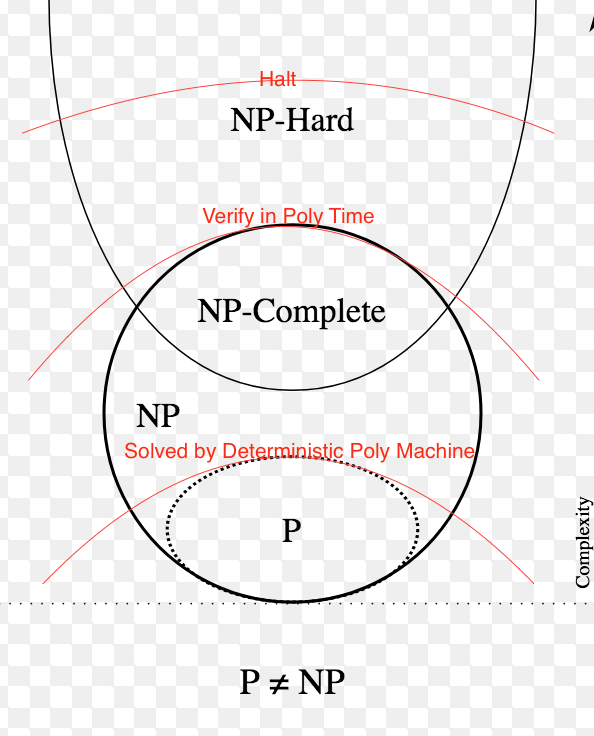
\includegraphics[scale=0.5]{NP.png}
    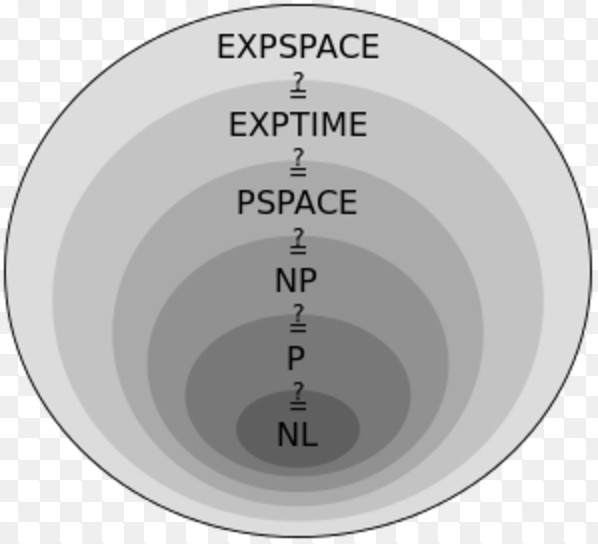
\includegraphics[scale=0.5]{PSPACE.png}
\end{figure}
\subsection{Axiom Systems}
\par We define an axiom system $K_n$, which characterizes Kripke structures for knowledge. $K_n$ consists of two axioms: \\
\par A1. All instances of tautologies of the propositional calculus
\par A2. $(K_i(\phi)\land K_i(\phi\Rightarrow\psi))\Rightarrow K_i(\psi),i=1,...,n$ \\
\par $K_n$ also consists of two rules: \\
\par R1. From $\vdash\phi$ and $\vdash\phi\Rightarrow\psi$ infer $\vdash\psi$
\par A2. From $\vdash\phi$ infer $\vdash K_i(\phi)$ \\
\par Besides Axioms that $K_n$ consists of, there are also other ways to characterize knowledge: \\
\par A3. $K_i(\phi) \Rightarrow \phi$, which states that only true facts can be known. This is similar to what we discussed in class as $\square\phi \implies \phi$ for T axiom in normal modal logic.
\par A4. $K_i(\phi) \Rightarrow K_i(K_i(\phi))$, which is the positive introspection axiom, which states that an agent knows what fact he knows. This is similar to what we discussed in class as $\square\phi \implies \square\square\phi$ for 4 axiom in normal modal logic.
\par A5. $\lnot K_i(\phi) \Rightarrow K_i(\lnot K_i(\phi))$, which is known as the negative introspection axiom, saying that an agent knows what facts he does not know. This is rejected by philosophers as we discussed in class.
\par A6. $\lnot K_i(false)$, saying an agent does not know inconsistent facts. This is similar to N axiom discussed in class.\\
\par Specifically, $K+A3$ has been called $T$, $T+A4$ has been called $S4$, $S4+A5$ has been called $S5$, and $K+A4+A5+A6$ has been called $KD45$.
\subsection{Correspondence between Model Structures and Axioms}
\par We say that a structure $M$ is a model of $K_n$ if every $K_n$-provable formula is valid in $M$. Ans similarly, $M$ is a model of $T_n, S4_n, S5_n, KD45_n$, if if every $T_n, S4_n, S5_n, KD45_n$-provable formula is valid in $M$, respectively. 
\par Since $K_n$ is a sound and complete axiomatization with respect to $M$(we have shown similar proof of soundness and completeness of system K in class), we can conclude that: \\
\par $T_n$ is a sound and complete axiomatization with respect to $M^r$.
\par $S4_n$ is a sound and complete axiomatization with respect to $M^{rt}$.
\par $S5_n$ is a sound and complete axiomatization with respect to $M^{rst}$.
\par $KD45_n$ is a sound and complete axiomatization with respect to $M^{elt}$.\\
\par We can observe that these four correspondence are corresponding to what we discussed in class. For example, for $T_n$, every reflexive structure satisfies all the axioms of $T_n$ and thus is a model of $T_n$. $T_n$, specifically, is $K+A3$, and $A3$ is analogous to the T axiom in normal modal logic, which also perfectly corresponds to reflexivity that was proven in class. As a nother instance, $S4_n$ has the rule $A4$ added, which refers to 4 axiom in normal modal logic. 
\par The only difference between such correspondences here and correspondence in normal modal logic is that we involve multiple agents here. However, we just modify $M$ that was discussed in class to be $M^r=(S,\pi,K_1^r,...K_n^r)$. As long as each of $K_i$ as accessive relations or epistemic relations are reflexive themselves, such proof can be considered as the same process. \\
\par Before going to complexity discussion, here are two important propositions to keep in mind: \\
\par If a formula $\phi$ is $S5$ consistent, then $\phi$ is satisfiable in a structure $M=(S,\pi,K_1)$, where $K_1$ is universal. 
\par If a formula $\phi$ is $KD45$ consistent, then $\phi$ is satisfiable in a structure $M=(\{s_0\}\cup S,\pi,K_1)$, where $S$ is nonempty and $K_1 = \{(s,t): s\in \{s_0\}\cup S, t\in S\}$ \\
These are provable and important for differentiating there complexity from $K,T,S4$.
\section{Deciding the Validity of Formulas}
\par Now it comes to the meat of the paper that the validity problem for $M,M^r,M^{rt},$\\$M^{rst},M^{elt}$ are provable.
\subsection{Validity and Satisfiability}
\par We consider how validity and satisfiability are defined differently from what we discussed in class. Here, validity and satisfiability are defined as follows: \\
\par Validity: $\phi$ is valid in $M$, if $(M,s)\vDash \phi$ for every state $s\in S$. Written as $M\vDash \phi$.\\We say $\phi$ is valid with respect to class $M$, if $\phi$ is valid in all structures in $M$.
\par Satisfiability: $\phi$ is satisfiable in $M$, if $(M,s)\vDash \phi$ for some state $s\in S$.\\We say $\phi$ is satiafiable with respect to class $M$, if $\phi$ is valid in some structures in $M$.
\par It is important to note, same as what is discussed in class, that $\phi$ is valid in $M$ iff $\lnot\phi$ is not satisfiable in $M$. So validity and satisfiability are regarded as complementary problems, and this point will be revisited in section 4.
\subsection{Decidability of $M_n$ and the Provability for $K_n$}
\par In order to know if the validity problem for $M_n$ are the probability problem for $K_n$ are decidable, we have to come with two observations: \\
\par First, given a structure $M$ and a formula $\phi$, there is an algorithm for checking if $\phi$ is satisfied in $M$ that runs in time $c*(|M|*|\phi|)$:
\par This is because we have to check at each state whether $\phi$ is true. To check on a single state whether $\phi$ is true, we consider all the subformulats of $\phi$, and the number of subformulas $Sub(\phi) \leq |\phi|$. So running time for checking single state is $O(|\phi|)$. And there are $|M|$ states in total, so the time will be in $O(|M|*|\phi|)$. The only part that is different from what we discussed in class is that $\phi$ involves relations of knowledge $K$. However, this is not a big problem since each $K_i(\psi)$ can be carried out in time at most of $O(|M|)$, by tracing back to $t$, if $(s,t)\in K_i$. Overall, the time is still polynomial. \\
\par Second, If $\phi$ is $K_n$ consistent then $\phi$ is satisfiable in a structure in $M_n$ with at most $2^{|\phi|}$ states where every primitive proposition which is not a subformula of $\phi$ is false at every state:
\par Proof: Let $Sub(\phi)^+$ consist of all the subformulas and their negations. Let $Con(\phi)$ be a set of maximal $K_n$ consistent subsets of $Sub(\phi)^+$. A member that belongs to $Con(\phi)$ is either $\psi$ or $\lnot\psi$ for all formula $\psi$ which is a subformula of $\phi$. We can assign 0 or 1 to true or false of such $\psi$ in a member of $Con(\phi)$. So we can easily deduce that $|Con(\phi)|$ is at most $2^{|\phi|}$, because number of $\psi$ is $|Sub(\phi)|\leq |\phi|$. \\ 
\par So we just construct $2^{|\phi|}$: this many $M_n$ and in each structure we construct, we use the checking algorithm mentioned in the first part to determine whether $\phi$ is satisfiable. This procedure is not different from what is discussed in class except for involving more agents during the checking algorithm. But satisfiability can still be decided in finite time, and thus validity can be decided for $K_n$.
\subsection{Extending Decidability to $T_n, S4_n, S5_n, KD45_n$}
\par Not only in the case of $K_n$, we can decide whether a formula $\phi$ is provable, similarly, we can decide whether a formula is provable, thus determining validity for $T_n, S4_n, S5_n, KD45_n$:
\par This is because during the model checking process, if we restrict our attention to particular structures, we can slightly modify the algorithm to check whether $\phi$ holds at a particular state $s$ in $M$. It basicly undergoes the same process without affecting the complexity.\\
\par Thus, validity problem for $M,M^r,M^{rt},M^{rst},M^{elt}$, with respect to $K_n, T_n,$\\$S4_n, S5_n, KD45_n$ are all decidable.
\section{Deciding the Satisfiability of Formulas with Respect to Complexity Classes}
\par We are interested in comparing difficulties of determining satisfiability of a given fomula $\phi$ over different classes of models in this section. Specifically, we consider $K_n, T_n, S4_n, S5_n, KD45_n$ with one or more agents. If not specified, it is referred to single agent case.
\subsection{Complexity Classes and Cook's Theorem}
\par Usually the difficulty of determining if a candidate belongs to a set is measured under time and space required. In this section we are going to show that $S5,KD45$ belong to $NP-complete$ complexity class whereas $K,T,S4,S5_2,KD45_2$ belong to $PSPACE-complete$ complexity class. \\
\par It is important to know Cook's Theorem beforehand:
\par The problem of determining whether a formula of propositional logic is satisfiable is NP-hard. \\
\par Another fact to notice is that given a complexity class $C$, the class $co-C$ includes all the sets whose complement is a member in $C$. So, since validity and satisfiability are complementary problems, and since satisfiability is NP-complete, validity if co-NP-complete as a result.
\subsection{NP-completeness for $S5, KD45$}
\par Here, we prove the $NP-complete$ tight bound of $S5$'s satisfiability given formula $\phi$ as a representation.
\subsubsection{Lower Bound for $S5$}
\par By Cook's Theorem, deciding $S5$ satisfiability is $NP-hard$, as hard as $NP$, because propositional calculus is part of $S5$.
\subsubsection{Upper Bound for $S5$}
\par As what we discussed in Section 2, If a formula $\phi$ is $S5$ consistent, then $\phi$ is satisfiable in a structure $M=(S,\pi,K_1)$, where $K_1$ is universal, It is provable that an $S5$ formula $\phi$ is satisfiable iff it is satisfiable in a structure in $M^{rst}$ with at most $|\phi|$ states.
\par Now we prove that such decision problem is actually in $NP$:
\par We do this by "guessing" a structure $M$ non deterministically with at most $|\phi|$ states, suppose the formula given is $\phi$. Say $M=(S,\pi,K)$, and $S$ contains at most $|\phi|$ states, since $K$ doesn't leave room for us to "guess", we only have $\pi$ needing to "guess". We "guess" the truth value of $\pi(s)(q)$. This can be done at $O(|\phi|^2)$ non deterministically, because we have $|\phi|$ choices for both $s,p$. Then we can use the checking algorithm discussed in section 3 to know whether $\phi$ is satisfied in such guessed structure. 
\par This is exactly what is defined as NP problem discussed in section 2. 
\subsubsection{Tight Bound for $S5$}
\par So, since deciding $S5$ satisfiability is both $NP-hard$ and $NP$, we can conclude that such problem is in $NP-complete$ class.
\subsubsection{Extending to $KD45$}
\par Similarly, by proving based on another key proposition from section 2, we can prove essentially the same result for $KD45$: a $KD45$ formula $\phi$ is satisfiable iff it is satisfiable in a structure in $M^{elt}$ with at most $|\phi|$ states.
\subsection{PSPACE-completeness for $K,T,S4,S5_2, KD45_2$}
\par We first use $K_n$ system as an example to show that it belongs to $PSPACE-complete$ class.
\subsubsection{Lower Bound for $K$}
\par As shown from section 3, if a formula $\phi$ is $K_n$ satisfiable then the satisfiability takes place in a structure of size $\leq 2^{|\phi|}$. However, as a comparison, $S5$ satisfiablility takes place in a structure of size of at most $|\phi|$. This indicates the reason why $K$ is not able to give an NP decision procedure for its satisfiability is that checking whether $\phi$ is satisfied at some state $s$ cannot be done deterministically in polynomial time.
\par Why is this the case? Briefly, according to what Ladner says, we consider quantified boolean formulae(QBF) in the form of $Q_1p_1Q_2p_2...Q_mp_mA'$, where $Q_i \in \{\forall,\exists\}$, and $A'$ is a propositional formula whose only primitive propositions are among $p_1...p_m$. We determine the truth of such QBF by replacing each subformula $\forall$ by $\land$, $\exists$ by $\lor$. In the case of $S4$, suppose we are given a QBF, we construct $\phi$ like a binary tree accordingly by $d_0\land\lnot d_1\land K(depth\land determined \land branching_A \land (d_m\Rightarrow A'))$, where $d_i$ is true iff we are at a depth $\geq i$. "Determined" means the truth value of $p_i$ is determined by depth $i$ in the tree, such that if $p_i$ is true at depth $j \geq i$ of node $s$, then $p_i$ is true for all successors of $s$. "Branching" means it is possible two have two successors at next depth such that $p_{i+1}$ is true and false, respectively. 
\par So we can see $\phi$ is satisfiable in a structure if $A$ is true. And since the size of $\phi$ is in polynomial of the size $A$, $S4$ satisfiability is taking at least as much space as $PSPACE$, so it is a $PSPACE-hard$ problem.
\par As for the lower bounds construction for $S5_2$, we can modify the structure $M^{rt}$ from $S4$ to get $M_2^{rst}$, and thus providing the same lower bound, details are omitted. One of the steps is that we replace every $K$ edge in $M$ by two edges, one for $K_1$ and the other for $K_2$. And then define $K_1$ and $K_2$ to both be $r,s,t$ closures $\{(s_{(s,t)},t: (s,t)\in K)\}$. The same underlying idea is for $KD45_2$. This invariantly shows that decidining satisfiability of $KD45_2$ is also a $PSPACE-hard$ problem.
\subsubsection{Upper Bound for $K$}
\par We argue for the upper bound for $K$ as PSPACE-complete, that is, can be solved using an amount of memory that is polynomial in the input length, by employing the tableau method.
\par The key lemma here is that the formula $\phi$ is $K_n$ (resp. $T_n,S4_n,S5_n,KD45_n$) satisfiable iff there is a propositional $K_n$ (resp. $T_n,S4_n,S5_n,KD45_n$) tableau for $\phi$.
\par A $K_n$ tableau is a tuple $T=(S,L,K_1,...,K_n)$ where $S,K_i$ are same as modals, and $L$ is the labeling function regarding each state $s\in S$.
\par $K_n$ tableau includes formulas that $L(s)$ is a propositional tableau without contradiction of propositions.
\par $K_i \psi \in L(s), (s,t)\in K_i$, then $\psi \in L(t)$.
\par $\lnot K_i \psi \in L(s)$, then $\exists (s,t)\in K_i and \lnot \psi \in L(t)$.
\par Note that $T$ is a $K_n$ tableau for $\phi$ if $T$ is a $K_n$ tableau and $\phi \in L(s)$ for some $s\in S$. 
\par A $T_n$ tableau takes reflexity in addition: if $K_i \psi \in L(s)$, then $\psi \in L(t)$.
\par Respectively, A $S4_n, S5_n$ tableau takes transitivity, seriality in addition, and a $KD45_n$ tableau takes euclidean property plus transitivity in addition to a $K_n$ tableau.
\par In the following discussion, we show how to construct a $K_n$ tableau for $\phi$ and see if the construction is successful in order to tell if $\phi$ is $K_n$ satisfiable. Then we prove that there is a verification process that takes space polynomial to input size $|\phi|$ to tell whether construction is successful, which indicates $K_n$ satisfiability problem is in complexity class of $PSPACE$. Given this result, we arrive at a tight bound for such problem as $PSPACE-complete$ problem.
\subsubsection{Tight Bound for $K$}
\par Here's the brief summary of construction of such tableau given:
\begin{verbatim}
    Step1: Construct a tree with single node root
    Step2: Repeat until non of (a)-(d) applies:
        (a). Forming a propositional tableau: if s is a leaf, 
        L(s) is not inconsistent, 
        L(s) is not formed completely, p is the least witness 
        (as defined in the original 
        paper):
            i. If p is !!p',create successor s' of s 
            such that L(s')=L(s)U{p'}
            ii.If p is p'Vp'',create successor s' of s 
            such that L(s')=L(s)U{p',p''}
            iii.If p is !(p'&p''),create successor s',s'' of s 
            such that L(s')=L(s)U{!p'},
            L(s'')=L(s)U{!p''}
        (b). Forming a fully expanded tableau
        (c). Creating successor nodes
        (d). Marking nodes "satisfiable": 
    Step3: If the root is satisfiable, return satisfiable,
        otherwise return unsatisfiable
        (some details are omitted)
\end{verbatim}
\par (An example of $K_n$ tableau construction for $\phi_0 = (p\land \lnot(p\land q))\land (K_1\lnot p \land \lnot K_1K_2q)$ is shown on the top of next page.)
\begin{figure}[h]
    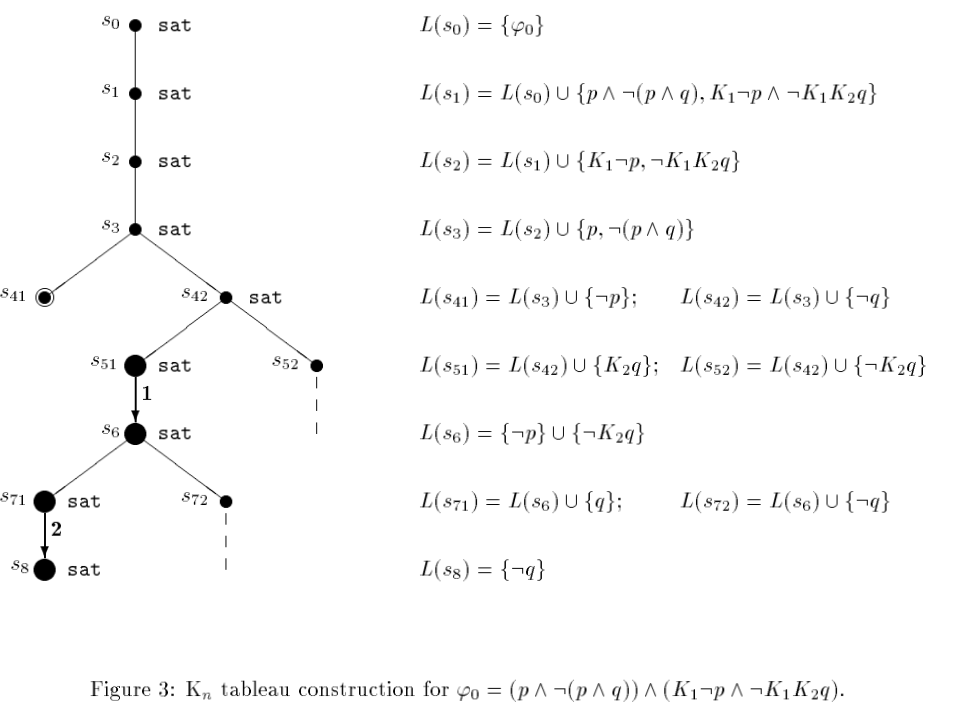
\includegraphics[scale=1]{EXAMPLE.png}
\end{figure}
\par It is proven that such construction will eventually terminate, and let's prove the correctness of the algorithm:
\par $"\Rightarrow"$: If the construction for $\phi$ returns "satisfiable", then there exists a $K_n$ tableau for $\phi$, by the key lemma, $\phi$ is $k_n$ provable(satisfiable).
\par $"\Leftarrow"$: Prove by contrapositive. If the root is not marked "satisfiable" by the algorithm, then $\lnot \phi$ is provable. Specifically, if the root is not marked "satisfiable", thus the conjunction of all the formulas $\psi$ in $L(root)$ is inconsistent, and then $\phi$ is not provable in $K_n$.(this can be proven by induction on the height of $root$ using bottom leaves as base cases: If $h=0$, then $L(s)$ is either inconsistent(not marked "satisfiable") or it has no formulas of form $\lnot K_i\phi$ (marked "satisfiable"). If $h>0$, $s$ is marked "satisfiable" iff one of its successors is marked "satisfiable"). So if $\phi$ is $k_n$ provable, the root is marked "satisfiable" by the algorithm.
\par Thus the construction for $\phi$ returns "satisfiable" iff $\phi$ is $k_n$ satisfiable.
\par The basic idea for this tableau construction algorithm is to permute, and see if there is any possible way to make $\phi$'s "nature" consistent.\\
\par There's an algorithm deciding satisfiability of $K_n$ formula occupying polinomial space:
\par How: A state $s$ only needs to use $3hm+m$ bits in total to store satisfiability states, where $h$ is the height of the tree after construction terminates, and $m$ is $|\phi|$. specifically, We use $m$ bits to store $\phi$, and $3hm$ bits to store information below it. We can use $2m$ bits to record information of $Sub^+(\phi)$ at a successor $s'$,(setting 1 as T and 0 as F at the corresponding bit, since there are at most $2m$ subformulas in $Sub^+(\phi)$), and $s'$ also keeps $m$ bits to store what nodes have yet explored. Since we only care about the final information stored at root $s$, we can reuse space over and over, ignoring the information stored at subnode's subnodes.
\par So we can verify if $\phi$ is satisfiable using space $O(m^3)$, which is polynomial.
\par This show s $K_n$ satisfiability problem is in $PSPACE$. Given the lower bound, we can conclude that $K_n$ satisfiability problem is in $PSPACE-complete$.
\subsubsection{Extending to $T,S4,S5_2, KD45_2$}
\par We can easily modify the procedure from $K_n$'s algorithm to make it work for $T_n$ by modifying some step 2(d) from the construction of tableau.
\par Similarly, we can modify the algorithm accordingly to construct $S4, S5_2, KD45_2$ tableau. Details are omitted here.
\par It is also proven that there exists an algorithm for deciding satisfiability of $S4_n$ formulas that runs in polynomial space: 
\par We show by induction on the height $h$ of a node $s$. We suppose $X$ is a list of labels appeared in ancestors of $s$. In this case, if we start the tableau construction with $L(s)$ as such node's label, we can determine how the node will be marked taking at most $(2h+3)*|\phi|+c+|X|$ bits of space. According to the fact that a node has at most $m^4$ ancestors, and requirement of storage for each label is $2m$ same as before, we can compute the labeling in polynomial space of $O(m^5)$ bits.
\par Similarly we can prove the existence of algorithm for deciding satisfiability of $T_n, S5_2, KD45_2$ formulas that runs in polynomial space(for example, an algorithm running in $O(m^2)$ bits for $S5_2$).
\par Finally, we can conclude that $T,S4,S5_2, KD45_2$ satisfiability problems are also in $PSPACE-complete$ complexity class.
\par The key reason to make deciding satisfiability for $S5,KD45$ modal logics in a much "quicker" class than the others' is the fact that we only need to verify them on a model with at most $|\phi|$ states, guaranteeing polynomial time verification whereas other 5 only guaranteeing polynomial space verification.
\section{Conclusion}
\par In this paper, we went over basic semantics of epistemic logic incorporated with multiple agents, and discovered the similarities shared with correspondence theories discussed in class. We identified axiom systems regarding ways to characterize knowledge.
\par We then identified and distinguished definitions of decidability, determinism, basic complexity classes. Then we examined decidability of validity of epistemic modal logics with multiple agents involved and how the involvements of multiple agents affect the decidability of validity for a given formula. The conclusion is such involvement may add complexity but it will not affect successfully deciding if a given formula is valid.
\par We then went into steps in deciding the satisfiability of formulas and attributing $K, S5, KD45, T,S4, S5_2, KD45_2$ into different complexity classes and prove that they meet the requirements of respective complexity classes' tight bounds. We also found that the involvement of multiple agents actually adds complexity in deciding the satisfiability, and that deciding if a given formula is satisfied is more complex if epistemic relation is under $K, T,S4,S5_2, KD45_2$ systems. 
\par Besides what we discussed so far, topics such as knowledge common to a group of agents as well as distributed knowledge are also interesting to be modeled and their complexities are meaningful to analyze, which could provide practical use in lots of areas, such as computer science. Moreover, broader range of modal logics such as $KB, KDB$ or temporal modal logics are good models to be analyzed of their complexity. The analyze can also involve analyzing probability under randomized algorithms. 
\section{References}
\begin{flushleft}
Joseph Y, Halpern, Yoram Moses, A guide to completeness and complexity for modal logics of knowledge and belied, 1996 \\ \\
\end{flushleft}
Lihn Anh Nruyen, On the Complexity of Fragments of Modal Logics, 2005
\end{document}
